\graphicspath{{chapters/colors/}}

Приведем пример применения UMAP на малой выборке.

Пусть у нас есть выборка из различных цветов, представленных в RGB-выражении. Соответственно, у нас имеется три признака: Red, Green, Blue.
\setlength{\extrarowheight}{2mm}
\begin{center}
\begin{multicols}{2}
	\begin{tabular}{c|c|c|cp{15mm}}
		& Red & Green & Blue & \\
		\cline{1-4}
		1 & 140 & 90 & 180 & \cellcolor[RGB]{140, 90, 180}\\
		\cline{1-4}
		2 & 249 & 132 & 229 & \cellcolor[RGB]{249, 132, 229}\\
		\cline{1-4}
		3 & 255 & 0 & 0 & \cellcolor[RGB]{255, 0, 0}\\
		\cline{1-4}
		4 & 191 & 34 & 51 & \cellcolor[RGB]{191, 34, 51}\\
		\cline{1-4}
		5 & 100 & 28 & 52 & \cellcolor[RGB]{100, 28, 52}\\
		\cline{1-4}
		6 & 0 & 47 & 85 & \cellcolor[RGB]{0, 47, 85}\\
		\cline{1-4}
		7 & 0 & 0 & 255 & \cellcolor[RGB]{0, 0, 255}\\
	\end{tabular}\\
	\begin{tabular}{c|c|c|cp{15mm}}
		& Red & Green & Blue & \\
		\cline{1-4}
		8 & 66 & 170 & 255 & \cellcolor[RGB]{66, 170, 255}\\
		\cline{1-4}
		9 & 0 & 110 & 126 & \cellcolor[RGB]{0, 110, 126}\\
		\cline{1-4}
		10 & 30 & 80 & 69 & \cellcolor[RGB]{30, 80, 69} \\
		\cline{1-4}
		11 & 48 & 186 & 143 & \cellcolor[RGB]{48, 186, 143}\\
		\cline{1-4}
		12 & 20 & 218 & 81 & \cellcolor[RGB]{20, 218, 81}\\
		\cline{1-4}
		13 & 0 & 255 & 0 & \cellcolor[RGB]{0, 255, 0}\\
		\cline{1-4}
		14 & 255 & 255 & 0 & \cellcolor[RGB]{255, 255, 0}\\
	\end{tabular}
\end{multicols}
\end{center}

Данные находятся в трехмерном пространстве. Мы можем изобразить их исходное состояние:
\begin{center}
	\begin{figure}[H]
		\noindent \centering {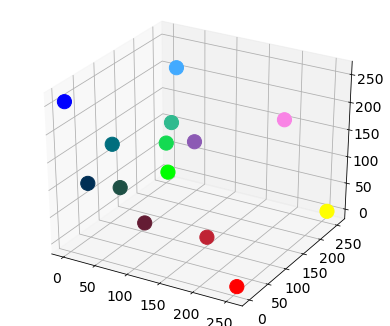
\includegraphics[width = 0.4\textwidth]{3Dcolors.png}}
	\end{figure} 
\end{center}

Попробуем теперь перевести их в 2-мерное пространство. Подберем гиперпараметры:
\begin{itemize}
	\item \verb|metric| --- признаки объектов заданы в числовом виде $\Rightarrow$ можно использовать евклидову метрику $\Rightarrow$ \verb|metric="euclidean"| (по умолчанию)
	\item \verb|n_components| --- мы хотим получить двумерное пространство $\Rightarrow$ \verb|n_components=2| (по умолчанию)
	\item \verb|min_dist| --- посмотрим на разные варианты, чтобы посмотреть и локальную, и глобальную структуру данных: $\{0.1, 0.3, 0.6, 1.0\}$
	\item \verb|n_neighbors| --- сложно подобрать данный гиперпараметр сразу, рассмотрим несколько вариантов: $\{2, 3, 8\}$
\end{itemize}

Для данной выборки не нужна предварительная обработка, поскольку все признаки определяют одну и ту же величину --- интенсивность цвета.
Запустим UMAP и посмотрим на результаты. Уберем оси, так как они показывают лишь значение некоторых абстрактных признаков, которые подобрал UMAP и не дают никакой полезной информации:
\begin{center}
\begin{tabular}{c|c|c|c}
\arrayrulecolor[rgb]{0.8,0.85,1}
	& \verb|n_neighbors=2| & \verb|n_neighbors=3| & \verb|n_neighbors=8| \\
	\hline
	\begin{sideways} \verb|min_dist=0.1| \end{sideways} & \includegraphics*[width = 0.18\textwidth]{0,1colors2.png} & \includegraphics*[width = 0.18\textwidth]{0,1colors3.png} & \includegraphics*[width = 0.18\textwidth]{0,1colors8.png} \\
	\hline
	\begin{sideways} \verb|min_dist=0.3| \end{sideways} & \includegraphics*[width = 0.18\textwidth]{0,3colors2.png} & \includegraphics*[width = 0.18\textwidth]{0,3colors3.png} & \includegraphics*[width = 0.18\textwidth]{0,3colors8.png} \\
	\hline
	\begin{sideways} \verb|min_dist=0.6| \end{sideways} & \includegraphics*[width = 0.18\textwidth]{0,6colors2.png} & \includegraphics*[width = 0.18\textwidth]{0,6colors3.png} & \includegraphics*[width = 0.18\textwidth]{0,6colors8.png} \\
	\hline
	\begin{sideways} \verb|min_dist=1.0| \end{sideways} & \includegraphics*[width = 0.18\textwidth]{1,0colors2.png} & \includegraphics*[width = 0.18\textwidth]{1,0colors3.png} & \includegraphics*[width = 0.18\textwidth]{1,0colors8.png} \\
\end{tabular}
\end{center}

При \verb|n_neighbors=2| четко видно деление цветов на разные кластера. При этом цвета примерно правильно распределились по оттенкам. Здесь UMAP учитывал связи только с ближайшими двумя соседями: искал похожих и ставил их рядом. Поэтому в кластерах примерно по три точки --- они все ближайшие соседи друг друга.

При \verb|n_neighbors=3| кластера начинают сливаться.  Если взять отдельный кластер из предыдущего случая, то теперь к нему присоединяются третьи по счету соседи тех объектов, которые в нем лежали, а за ними ближайшие соседи соседей. Поэтому здесь больше точек в кластерах при \verb|min_dist=0.1| и \verb|min_dist=0.3| и нет явных кластеров при \verb|min_dist>0.3| Но видны сходства с предыдущим относительным положением точек: зеленые лежат рядом друг с другом, темные точки по-прежнему близко.

При \verb|n_neighbors=8| сеть связей еще сильнее. Теперь можно разглядеть глобальную структуру и увидеть плавные переходы оттенков цветов, что напоминает цветовой спектр.

В целом, все три случая похожи на исходное трехмерное пространство. Точки, которые лежали рядом, по-прежнему являются соседями. При \verb|n_neighbors=2| они даже разбиваются на группы, которые можно также увидеть и в исходном пространстве, но менее явно. То есть UMAP также позволяет выполнить небольшой анализ --- он показывает нам взаимосвязи, которые мы не видели на исходных данных.
